\section{Page--Wootters and detector models for a two-level system}

\subsection{Detector models}

As we have seen in the previous sections,
proper elements of $\pwspace$,
localized in both space and time,
can be interpreted as ``events''
(as opposed to full history vectors, which instead describe the unitary evolution
of a quantum system \emph{at all times}).

The arrival of a particle at a detector
is a kind of event
of particular interest from the perspective of time
in quantum mechanics, for several reasons.

The first reason
is the direct connection with experiments,
``given the appalling evidence that time is also a random variable in the laboratories''
\parencite[\ch 4]{TQM2};
and because,
``{[as]} a matter of fact, a number of time observables are already routinely measured in laboratories,
for example arrival times in time-of-flight experiments,
but the theoretical foundation of these measurements is still being discussed''
\parencite[Preface to the First Ed.]{TQM1}.

The second reason is the existence of studies
about detector models which also investigate
time-of-arrival as a quantum observable,
as we have seen in Section \ref{sec:hist:detect}.
None of those works are explicitly
based on Page--Wootters relational model ---of which, to our knowledge,
there are no working examples of application to
time-of-detection problems in the current literature.
Section \ref{sec:absorption+pw} and the remainder of the chapter
will be devoted to bridging such gap
by implementing such application
and comparing
the results from the different models.
Some emphasis will be given to
\emph{discrete} relational time
using the techniques developed in Section \ref{sec:pw:qubit}.

One of the goals of this chapter
is indeed combining PW and detector models.

Another route is POVM, see Chap. \ref{ch:decohere} and \ref{ch:hist}.
Nonetheless, we know that a projective measurement on a bipartite system
can be regarded as a POVM
if we look at
on one part only (e.g. \cite{Paris2012}),
thus the clock space of the Page--Wootters mechanism, $\hilb{H}_T$,
can be regarded as a purification space \parencite{Paris2012} for the ``standard''
Hilbert space where the time-of-arrival POVM is defined,
and an interesting line of further research would be a more formal
study of the logical connection between the two approaches, based on this principle.
Both models respond to the issues raised by Pauli
by giving up
the pursuit of
a \emph{projective} measurement in the \emph{standard} Hilbert space,
and rather ``opening'' that Hilbert space in some sense.


\subsection{Comparison with the Page and Wootters formalism}
\label{sec:absorption+pw}

The detector absorption model in \cite{RuschhauptAbsorption} is not originally
based on the notion of quantum relational time. It is ``ordinary quantum mechanics''
in the sense that states are in $\hilb{H}_S$ with an external parameter time;
but, contrary to quantum mechanics, the potential can be \emph{complex},
causing the norm of the state vector to not be conserved (in fact, vanishing with time).
In other terms, the evolution is not unitary, even for a pure state.
Specifically, the Hamiltonian is corrected by an anti-hermitian term
that models the detector.

One may wonder whether a proper, normalized Page--Wootters ``position-time wavepacket''
(as described in Section \ref{sec:properpw})
can be used to describe \emph{the event of being detected} (or being absorbed).
It's expected to be peaked around the time when the absorption by the detector is maximum.

\citereset
In the detector model of \cite{RuschhauptAbsorption}, the detection
by absorption
corresponds to the \emph{decrease} in norm of the wavefunction.

Therefore we expect the following relation to be true:
\begin{equation}\label{eq:pwkiukas}
  \braket{\phi(t)} = -\dv{t}\norm{\psi_{\text{Kiukas}}(t)}^2 \text{,}
\end{equation}
both sides of which indicate probability of arrival at time $t$.
Here the function $\phi$ of time $t$ has to be intended in the sense of
\eqref{eq:pwphi}.

\citereset
Interestingly, the same paper provides a solution of \eqref{eq:pwkiukas}.
Despite not being based on the Page--Wootters model, eq. 9 in \cite{RuschhauptAbsorption}
equates the squared norm of a ``time representation'' wavefunction
to the opposite derivative of the squared norm of the ``absorbed wavefunction''.
It reads:
\begin{quote}
  We will associate with any wave function $\psi \in \hilb{H}$
  another wave function $\op{\psi}$,
  which is a function of time, so that
  $\abs{\op{\psi}(t)}^2$
  is the arrival probability density. In other words,
  $\op{\psi}$ is a wave function in a time representation. For each
  $t$, $\op{\psi}(t)$ lies in the original Hilbert space $H$.
\end{quote}
Therefore we ``translate''
$$\op{\psi}(t) \text{ into } \ket{\phi(t)}_S$$
and, consequently,
$$\abs{\op{\psi}(t)}^2 \text{ into } \braket{\phi(t)} \text{,}$$
in the language of the Page--Wootters model and within the notation
adopted.

\citereset
Using eq. 8 in \cite{RuschhauptAbsorption} and translating into our notation we have:
\begin{equation}\label{eq:phi_psi_kiukas}
  \op{\psi}(t) \eqbydef
  \ket{\phi(t)}_S =
  \begin{cases}
    \sqrt{\frac{2}{\hbar}} \op{D}^{1/2} \ket{\psi_{\text{Kiukas}}(t)}_S &\text{ if } t > 0 \\
    0 &\text{ otherwise. }
  \end{cases}
\end{equation}
Where at $t \le 0$ the interaction with the detector is yet to come,
but so it is, as a limit, for small values of $t>0$,
in other terms
$\lim_{t \to 0^{+}} \norm{\op{D} \ket{\psi_{\text{Kiukas}}(t)}} = 0$, thus avoiding the apparent discontinuity.

The corresponding Page--Wootters (proper) vector of $\pwspace$ is
\begin{equation}\label{eq:hatpsi:pw}
  \dket{\Phi} = \int \dd{t} \ket{t} \ox \op{\psi}(t) \,\text{,}
\end{equation}
to which the considerations of Section \ref{sec:for-normalized-elements}
and Section \ref{sec:for-normalized-elements} in terms of time--frequency
(or time--energy) uncertainty relation apply, with some analogy
to what \cite{RuschhauptAbsorption} does within its own framework
in relation to $\op{\psi}$ and its Fourier transform.

In that regard, the \eqref{eq:hatpsi:pw} can be reformulated
\begin{equation}
  \dket{\Phi} = \int \dd{\omega} \ket{\omega} \ox \mathcal{F} \op{\psi} (\omega) \,\text{,}
\end{equation}
where it is
\begin{equation}
  \mathcal{F} \op{\psi} (\omega) = - \frac{\sqrt[4]{2} i}{\sqrt{\pi} \left(- \omega^{2} + \sqrt{2} i \omega + 1\right)} \ket{1}
\end{equation}
---see notebook up to Eq.~\eqref{eq:fhatpsi1_omega} for details.


\citereset
\subsubsection{
  (Non-unitary) evolution without evolution:
  plugging the complex potential in the \emph{discrete} Page--Wootters model
}

Similarly to what seen in Section \ref{sec:building-the-discrete-pw-clock}, we build
the clock by defining ---and representing in a convenient basis---
the time operator and the corresponding frequency operator:
\begin{align}
  \op{T} \repr \frac{2\pi}{N}
  \begin{pmatrix}
    0           &       &       &       \\
                &1      &       &       \\
                &       &\ddots &       \\
                &       &       &N-1
  \end{pmatrix}
  &&
  \op{\Omega} = \frac{N}{2\pi} F^{\dagger}_{N} \op{T} F^{}_{N} \, \text{,}
\end{align}
where $F$ is, again, the discrete Fourier operator of order $N$.

Next we define the Wheeler--DeWitt operator $\mathbb{J}$ as in
\eqref{eq:pwHamiltonian}, but $\op{H}_S$ is replaced by the non-hermitian
Hamiltonian of the detector model
$\mathit{K}_S = \op{H}_S - \iu \op{D}_S$
\parencite{RuschhauptAbsorption},
where the subscript $_S$ has been added to stress
that they would act on the $\hilb{H}_S$ part
of the Page--Wootters' $\pwspace$ ``spacetime'':
\begin{equation}\label{eq:pwHamiltonian:nonUnitary}
  \mathbb{J} = \hbar\op{\Omega}\ox\idop_S + \idop_T\ox\qty(\op{H}_S -\iu \op{D}_S) \,\text{.}
\end{equation}
$\op{H}_S$ and $\op{D}_S$ are the same as $\op{H}$ and $\op{D}$
respectively from the \eqref{eq:complexpot}.

We then compute eigenvalues and eigenvectors of $\mathbb{J}$.
Eigenvectors associated to the eigenvalue $0$ will include
the history of the qubit over a ``period''
(of what would have been a periodic evolution, without the absorptive detector).

Eigenvectors associated to non-zero eigenvalues will need a ``phase correction'',
or energy shift\footnote{ Again, see also ref. \cite[\it ``The Zero-eigenvalue'']{Lloyd:Time}. }
as seen, for example, in \eqref{eq:comparison0} and \eqref{eq:comparison1}.
%% TODO? Examiners wanted more clarity ("proof"?). No time right now, and it is not referred anywhere.
%% So just rely on \cite[\it ``The Zero-eigenvalue'']{Lloyd:Time},
%% \eqref{eq:comparison0} and \eqref{eq:comparison1}.
%%
% Or, in a more compact form:
% \begin{equation}
%   \dket{n}_{\text{hist.}} = e^{-\iu \epsilon_n \op{T}} \ox \idop_S \dket{n}
%   \,\text{,}
% \end{equation}
% where $\epsilon_n$'s are eigenvalues of $\mathbb{J}$ and
% $\dket{n}$'s their corresponding eigenvectors.

\citereset
Linear combination of histories $\sum_n \alpha_n \dket{n}_{\text{hist.}}$
are also physically possible\footnote{
  As opposed to (linear combinations of) mere, uncorrected eigenstates of $\mathbb{J}$.
  Indeed, one may observe,
  at least in the case where $\mathbb{J}$ was hermitian,
  that $\setof{\dket{n}}$ is a basis
  of $\pwspace$ therefore
  $\sum_n \alpha_n \dket{n}$ would span \emph{all elements}
  of $\pwspace$ and the theory would not predict anything i.e.
  it would not discriminate unphysical histories.
}
and in fact we pick
one that ensure that the initial state ${}_{T}\bradket{0}{\Psi}$ is equal to $\ket{0}_S$
so to allow a comparison with the example in \cite{RuschhauptAbsorption}.
Such linear combination is not unique. For reasons of numerical stability,
a linear combination with coefficients in the order of 1 would be ideal if it exists.
In this particular problem, it does.
We simply scan, as a first attempt, all possible values ${}_{T}\bradket{0}{n} + {}_{T}\bradket{0}{m}$
to find a combination that is equal to $\ket{0}_S$
-- or maximizes the fidelity with that respect.\footnote{
  See the definition, and invocation, of the function \texttt{find_best()} in Appendix \ref{discrete-page-wootters-model}.
}

All the above numerical computation is implemented with \emph{NumPy} \parencite{comp:numpy},
particularly in appendix
\ref{discrete-page-wootters-model}.
The results are visualized in
Fig. \ref{fig:absorbed-qubit-components_pwlattice},
and are \emph{compatible} with the non-Page--Wootters
solution previously shown in Fig. \ref{fig:absorbed-qubit-components}.

\begin{figure}
  \centering
  \begin{subfigure}[b]{0.49\textwidth}
    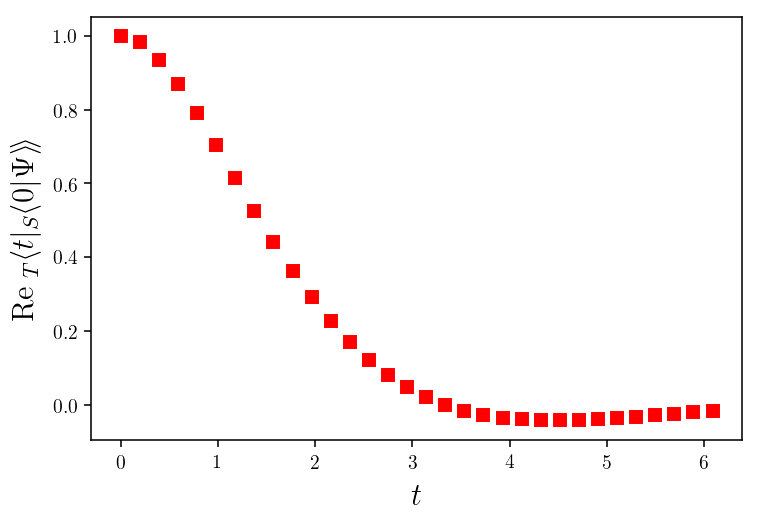
\includegraphics[width=\linewidth]{img/2ldetect/re_psi0_t_pwlattice.png}
    \subcaption{}\label{fig:absorbed-qubit-components_pwlattice:re0}
  \end{subfigure}
  \begin{subfigure}[b]{0.49\textwidth}
    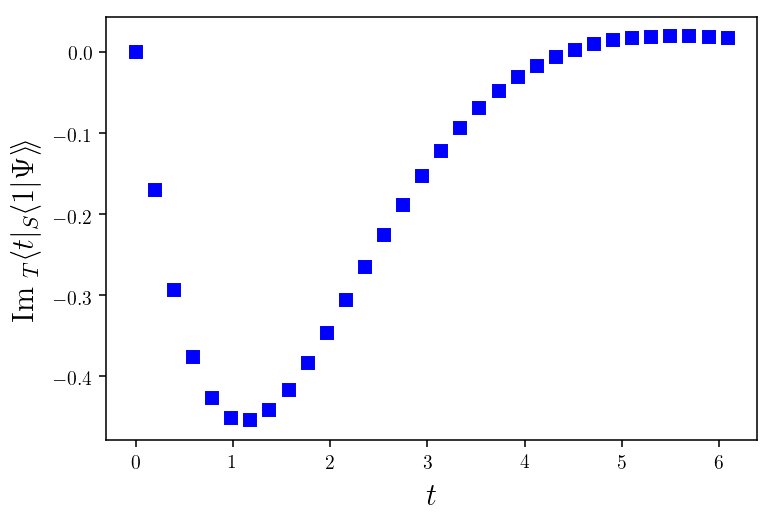
\includegraphics[width=\linewidth]{img/2ldetect/im_psi1_t_pwlattice.png}
    \subcaption{}\label{fig:absorbed-qubit-components_pwlattice:im1}
  \end{subfigure}
  \caption[
    Non-unitary ``evolution without evolution'' (discrete).
  ]{
    Non-unitary ``evolution without evolution''
    using the discrete Page--Wootters model,
    plugging in
    the complex potential of \cite{RuschhauptAbsorption}.
    The result is compatible with the continuous
    ``Schr\"odinger evolution''
    shown in Fig. \ref{fig:absorbed-qubit-components}.
    Note the different notation e.g.
    $\mathrm{Re}{\;}_{T}\hspace{-.2em}\left\langle t | {}_{S}\hspace{-.2em}\left\langle 0 | \Psi \right\rangle\hspace{-.17em}\right\rangle$
    to fit within the framework of the P--W space-time $\pwspace$.
  }
  \label{fig:absorbed-qubit-components_pwlattice}
\end{figure}

\subsubsection{Detection probability amplitude, time of arrival distribution}

In \cite{RuschhauptAbsorption} the probability of detection in time is given
by how fast the norm decreases i.e. $-\dv{\norm{\psi}^2}{t}$.
A ``wavefunction in time'', whose squared modulus equates the detection probability,
is introduced in eq. (8) therein:\footnote{
  Please note we are importing some notation from \cite{RuschhauptAbsorption} as per the symbol $\op{\psi}$,
  at variance to what generally adhered to in this work,
  where the ``hat'' ($\op{\;}$) denotes quantum observables and their corresponding operators.
}
\begin{equation}
  \op{\psi} = \theta(t) \sqrt{2/\hbar}\,\op{D}^{1/2}\,\psi
\end{equation}
In Page--Wootters terms, this translates into applying
$\theta(\op{T}) \ox \sqrt{2/\hbar}\,\op{D}^{1/2}_S$
to the each history vector $\dket{n}_{\text{hist.}}$
(and their linear combinations).
The result is a detection-event \emph{proper} element of ${\pwspace}$
(that would be normalizable in a continuous, infinite-time model too):
\begin{equation}\label{eq:qubit_detection_wavefunction}
  \dket{\Phi_n} =
    \theta(\op{T}) \ox \sqrt{2/\hbar}\,\op{D}^{1/2}_S \dket{n}_{\text{hist.}} =
    \theta(\op{T}) e^{-i\epsilon_{n}\op{T}} \ox \sqrt{2\op{D}} \dket{n} \, \text{.}
\end{equation}
Given we are considering, in our discrete model, only an interval of time within $0$ and $2\pi$,
i.e. all non-negative times (or, more physically, only times when the detector is active),
the Heaviside function $\theta$ (of operator) can be omitted, and simply replaced
by the identity in time $\idop_T$.

Of course, for our problem, we take a linear combination
\begin{equation}
  \dket{\Phi} = \sum_n \alpha_n \dket{\Phi_n}
\end{equation}
where the coefficients $\alpha_n$ are the same that verified
(not necessarily uniquely)
the initial condition of the problem
$\ket{0}_S = {}_T\bradket{0}{\Psi} = \sum_n \alpha_n \, {}_T\bradket{0}{n}_{\text{hist.}} = \sum_n \alpha_n \, {}_T\bradket{0}{n}$.

\citereset
The vector $\dket{\Phi}$, proper element of $\pwspace$,
is the Page--Wootters counterpart of the function
``in time representation'' $\op{\psi}$,
as
described in \cite{RuschhauptAbsorption}. In formulas:
\begin{equation}
  \bradket{t}{\Phi} = \op{\psi}(t) \, \text{.}
\end{equation}

The ``detection wavefunction''~$\dket{\Phi}$ will always lie,
\emph{spatially},
in the space generated by $\ket{1}_S$, or in other terms:
\begin{equation}\label{eq:detect_prob_ampl_only_on_1}
  \prescript{}{T}{\bra{t}}\prescript{}{S}{\bradket{0}{\Phi}} = 0 \text{,} \quad \forall t \, \text{.}
\end{equation}
The linear space of $\ket{1}_S$ is the ``detectable area'' of the qubit
in this problem, and
$\dket{\Phi}$ is essentially the result of the action of the operator $\op{D}$,
that filters non-detectable components out from any vector of $\hilb{H}_S$.

We derive the components of $\dket{\Phi}$ numerically in Section \ref{detection-event},
where they are encoded in the array \texttt{prob_detect_v}.
We observe therein that the \eqref{eq:detect_prob_ampl_only_on_1} is confirmed,
and that ${}_T\!\bra{t} {}_S\!\bradket{1}{\Phi}$ is proportional
to the $\ket{1}$-component of the evolution of the qubit (history $\Dket{\Psi}$)
at any time $t$
(%
  which is not surprising, being $\sqrt{2/\hbar}\op{D}^{1/2}$ of the form
  $\scriptsize \left[\begin{matrix}0 & 0\\0 & \kappa \end{matrix}\right]$%
).
In more formal terms:
\begin{equation}\label{eq:detect_prob_amplitude_proportional}
  \exists \kappa: \: {}_T\!\bra{t} {}_S\!\bradket{1}{\Phi} = \kappa \cdot {}_T\!\bra{t} {}_S\!\bradket{1}{\Psi} \; \forall t \text{,}
\end{equation}
which, algebraically, is almost obvious, given the considerations above.
However, it is worth noting that the expression on the right side
(up to a factor $\kappa$) is, at each $t$,
an ordinary quantum mechanical probability amplitude
(probability amplitude of being $\ket{1}$ rather than $\ket{0}$);
while the expression on the left side, as a function of $t$,
is a probability amplitude \emph{in time}.
Even when normalized (in the probabilistic sense), the two expressions
are proportional but not equal (hence the factor $\kappa$).
This is because the expression on the right must be normalized
so that, at each $t$,
${ \abs{ {}_T\!\bra{t} {}_S\!\bradket{0}{\Psi} }^2 + \abs{ {}_T\!\bra{t} {}_S\!\bradket{1}{\Psi} }^2 = 1 }$
(or, actually, equal to $ \braket{\psi(t)} \leq 1$, the ``lossy norm'' due to absorption).
Whereas the expression on the left must be normalized so that
$\sum_t \norm{ {}_T\!\bradket{t}{\Phi} }_S^2 = P$,
where $P$ is the total probability that the detection/absorption happens at any time,
and it's equal to $1$ for an ideal detection.

\citereset
The probability of detection in time is shown in Fig. \ref{fig:2l_pw_detect_prob_t}
and is \emph{consistent} with the result of
the continuous and not explicitly Page--Wootters model of
\cite{RuschhauptAbsorption} (see Fig. \ref{fig:absorbed-qubit-normalization-loss:t}).

Switching to the frequency (and, therefore, \emph{energy}) domain,
the discrete Fourier transform yields another proper vector
$\Dket{\tilde{\Phi}}$ of $\pwspace$:
\begin{equation}
  \Dket{\tilde{\Phi}} = F \ox \idop_s \dket{\Phi} \, \text{.}
\end{equation}
This vector numerical values, taken pairwise
(or by groups of 3 for a qutrit etc.)
are the components in the computational basis
of the kets $\ket{\tilde{\phi}(\omega)} \in \hilb{H}_S$
such that
\begin{equation}
  \dket{\Phi} = \sum_n \ket{t}\bradket{t}{\Phi} = \sum_{\omega} \ket{\omega}\bradket{\omega}{\Phi}
    = \sum_{\omega} \ket{\omega}_T \ox \ket{\tilde{\phi}(\omega)}_S \, \text{.}
\end{equation}

As a numerical array, $\Dket{\tilde{\Phi}}$ is the representation of $\Dket{\Phi}$
under the basis $\ket{\omega} \ox \ket{0,1}$ instead of $\ket{t} \ox \ket{0,1}$,
where the $\ket{\omega}$ constitute an eigenbasis of angular frequency $\op{\Omega}$.

\citereset
The squared norms $\braket{\tilde{\phi}(\omega)}_{\!S} = \norm{\braDket{\omega}{\Phi}}_S^2$
give the probability of detection in the frequency domain, which is plotted in
Fig. \ref{fig:2l_pw_detect_prob_omega} and, again, consistent
with Fig. \ref{fig:absorbed-qubit-normalization-loss:omega} i.e.
the result from the model of \cite{RuschhauptAbsorption}.

\begin{figure}
  \centering
  \begin{subfigure}[b]{0.49\textwidth}
    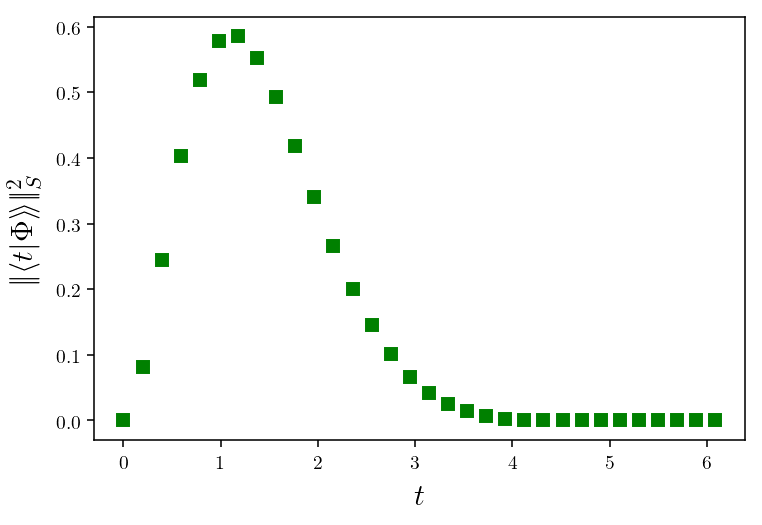
\includegraphics[width=\linewidth]{img/2ldetect/pw-detect-prob.png}
    \subcaption{}\label{fig:2l_pw_detect_prob_t}
  \end{subfigure}
  \begin{subfigure}[b]{0.49\textwidth}
    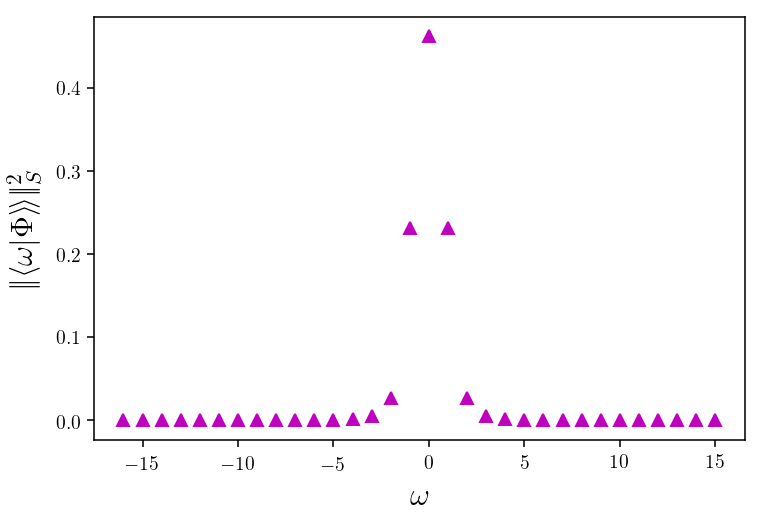
\includegraphics[width=\linewidth]{img/2ldetect/pw-detect-prob-ft.png}
    \subcaption{}\label{fig:2l_pw_detect_prob_omega}
  \end{subfigure}
  \caption[
    Arrival at the detector, probability distribution.
  ]{
    Arrival at the detector, probability distribution:
    \subref{fig:2l_pw_detect_prob_t} in the time domain
    and \subref{fig:2l_pw_detect_prob_omega} in the frequency domain.
  }
  \label{fig:2l_pw_detect_prob}
\end{figure}

\subsubsection{Time--energy uncertainty relation}

% In quantum systems described by a finite Hilbert space,
% uncertainty relations are quantified in terms of \term{entropies}
% of the canonically conjugate probability distributions
% ---see Section \ref{sec:finite_uncertainty} and references therein,
% in particular \cite{FiniteHilb}.

% In our example, the entropic uncertainty relation explicitly reads:
% \begin{multline}
%  S_T + S_{\Omega} =
%   -\sum_t \norm{\bradket{t}{\Phi}}_S^2 \ln \norm{\bradket{t}{\Phi}}_S^2
%   -\sum_{\omega} \norm{\bradket{\omega}{\Phi}}_S^2 \ln \norm{\bradket{\omega}{\Phi}}_S^2 \\
% %
%   = -\sum_{n=0}^{N-1} \left(\abs{\Phi_{2n}}^2 + \abs{\Phi_{2n+1}}^2\right) \ln \left(\abs{\Phi_{2n}}^2 + \abs{\Phi_{2n+1}}^2\right) \\
%     -\sum_{m=0}^{N-1}
%           \left(\abs{\tilde{\Phi}_{2m}}^2 + \abs{\tilde{\Phi}_{2m+1}}^2\right)
%       \ln \left(\abs{\tilde{\Phi}_{2m}}^2 + \abs{\tilde{\Phi}_{2m+1}}^2\right) \\
% %
%   \geq \ln N
% \end{multline}
% ---where we had computed previously the probability values in parenthesis.

% In Section \ref{jupy:entropic-uncertainties}, we numerically find that
% \begin{equation*}
%   S_{T} + S_{\Omega} \approx 1.14 \cdot \ln N
% \end{equation*}
% i.e. circa $14\%$ more than the theoretical minimal uncertainty.

% In terms of uncertainty relation based on standard deviations,
% which is the standard formulation, particularly for continuous distributions,
% and allows a comparison with \cite{RuschhauptAbsorption},
We compute numerically
\begin{equation}\label{eq:uncertainty-us}
  \sigma_{T} \sigma_{\Omega} \approx 0.716 \, \text{,}
\end{equation} \citereset
while \cite{RuschhauptAbsorption} finds
\begin{equation}\label{eq:uncertainty-them}
  \sigma_{T} \sigma_{\Omega} \approx 0.707 \, \text{.}
\end{equation}

The two models yield different predictions. A brief discussion follows.

Preliminarily, we should observe that the example in the paper
sets the optimal parameters to minimize the time--energy uncertainty
\emph{within the given constraints} of the particular physical system,
they do not necessarily achieve the theoretical Heisenberg minimum of
$\frac{\hbar}{2}$
(or $0.5$ in our numerical problem where $\hbar$ has been adimensionalized).
More notably, parameters therein have been chosen so to minimize
an alternative definition of time--energy uncertainty, $\expval{T}\sigma_E$,
deemed more meaningful within the physics of the particular system.

\citereset
Nonetheless, with minimal or not minimal uncertainty states (or ``histories''),
a comparison of such uncertainties between the discrete Page--Wootters model,
implemented here,
and the model in \cite{RuschhauptAbsorption},
can be performed:
the difference between the results in \eqref{eq:uncertainty-us}
and \eqref{eq:uncertainty-them} may be large enough to be not simply
due to numerical approximation. A further line of investigation
will involve increasing the resolution (number of levels) of the quantum clock.
If the discrepancy persists, an experimental verification
---as the one proposed in the paper itself---
will then be of
particular interest. The issue of discriminating different model of arrival time has
been tackled recently by other authors as well \parencite{Maccone_arrival}.
